\documentclass[margin=10pt]{standalone}
\usepackage{color,xcolor}
\usepackage{makecell}
\usepackage{tikz-qtree, tikz}
\usetikzlibrary{arrows.meta,bending}
\usetikzlibrary{calc,trees,positioning,arrows,chains,shapes.geometric,%
    decorations.pathreplacing,decorations.pathmorphing,decorations.markings,shapes,%
    matrix,shapes.symbols,positioning,angles,quotes,patterns}
\usepackage[utf8]{inputenc}

%See https://tex.stackexchange.com/a/29367/1952
\makeatletter
\tikzset{% customization of pattern
        hatch distance/.store in=\hatchdistance,
        hatch distance=5pt,
        hatch thickness/.store in=\hatchthickness,
        hatch thickness=5pt
        }
\pgfdeclarepatternformonly[\hatchdistance,\hatchthickness]{north east hatch}% name
    {\pgfqpoint{-1pt}{-1pt}}% below left
    {\pgfqpoint{\hatchdistance}{\hatchdistance}}% above right
    {\pgfpoint{\hatchdistance-1pt}{\hatchdistance-1pt}}%
    {
        \pgfsetcolor{\tikz@pattern@color}
        \pgfsetlinewidth{\hatchthickness}
        \pgfpathmoveto{\pgfqpoint{0pt}{0pt}}
        \pgfpathlineto{\pgfqpoint{\hatchdistance}{\hatchdistance}}
        \pgfusepath{stroke}
    }
\makeatother

\definecolor{myblue}{HTML}{0072BD}
\definecolor{mygreen}{HTML}{258F1B}
\definecolor{myred}{HTML}{C4000C}

\newcommand{\Ms}{\ensuremath{M_\mathrm{s}}} % Martensite start Temperature
\newcommand{\Mf}{\ensuremath{M_\mathrm{f}}} % Martensite finish Temperature
\newcommand{\As}{\ensuremath{A_\mathrm{s}}} % Austenite start Temperature
\newcommand{\Af}{\ensuremath{A_\mathrm{f}}} % Austenite finish Temperature

% \usetikzlibrary{decorations.pathreplacing,arrows,shapes,positioning,shadows,calc}
% \usetikzlibrary{decorations, decorations.text,backgrounds}
% \tikzset{every picture/.style={font issue=\footnotesize},
%     font issue/.style={execute at begin picture={#1\selectfont}}
% }

\begin{document}
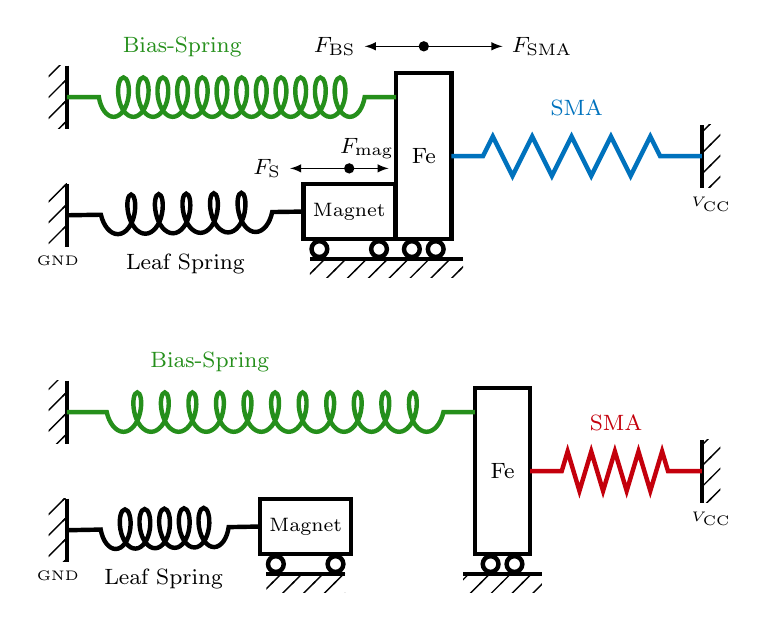
\begin{tikzpicture}[every node/.style={draw,outer sep=0pt,ultra thick,font=\footnotesize}]
\tikzstyle{sma-stretched}=[ultra thick,decorate,decoration={zigzag,pre length=4mm,post length=4mm,segment length=5mm, amplitude=2.5mm}]
\tikzstyle{spring}=[ultra thick,decoration={aspect=0.5,pre length=4mm,post length=4mm,segment length=2.5mm, amplitude=2.5mm,coil},decorate]
\tikzstyle{ground}=[pattern=north east hatch, hatch distance=3mm, hatch thickness=.5pt, fill,draw=none,minimum width=2mm,minimum height=0.1mm]

\tikzstyle{smalong}=[ultra thick,decorate,decoration={zigzag,pre length=4mm,post length=4mm,segment length=9mm, amplitude=2.5mm}]
\tikzstyle{springshort}=[ultra thick,decoration={aspect=0.5,pre length=4mm,post length=4mm,segment length=2mm, amplitude=2.5mm,coil},decorate]

\tikzstyle{sma}=[ultra thick,decorate,decoration={zigzag,pre length=4mm,post length=4mm,segment length=3mm, amplitude=2.5mm}]
\tikzstyle{spring-stretched}=[ultra thick,decoration={aspect=0.5,pre length=4mm,post length=4mm,segment length=3.5mm, amplitude=2.5mm,coil},decorate]

% \tikzstyle{ground}=[fill,pattern=north east lines,draw=none,minimum width=2mm,minimum height=0.1mm]
% \tikzstyle{damper}=[thick,decoration={markings,
%   mark connection node=dmp,
%   mark=at position 0.5 with
%   {
%     \node (dmp) [thick,inner sep=0pt,transform shape,rotate=-90,minimum width=15pt,minimum height=3pt,draw=none] {};
%     \draw [thick] ($(dmp.north east)+(2pt,0)$) -- (dmp.south east) -- (dmp.south west) -- ($(dmp.north west)+(2pt,0)$);
%     \draw [thick] ($(dmp.north)+(0,-5pt)$) -- ($(dmp.north)+(0,5pt)$);
% }
%   }, decorate]

    % SMA (Hot)
    \coordinate (Fe-Coord) at (0,0);
    \coordinate[left=of Fe-Coord,xshift=1.5pt] (Mag-Coord);

    \node[minimum width=20,minimum height=60, anchor=south] (Fe) at (Fe-Coord) {Fe};
    \node (ground) [ground,anchor=north,yshift=-0.25cm,minimum width=1cm] at (Fe.south) {};
    \draw[ultra thick] (ground.north east) -- (ground.north west);
    \draw [ultra thick] (Fe.south west) ++ (0.2cm,-0.125cm) circle (0.1cm)  (Fe.south east) ++ (-0.2cm,-0.125cm) circle (0.1cm);
    \node (groundL) at (Fe.east) [ground, xshift=-5cm, yshift=0.75cm, rotate=-90, minimum height=0.1mm, minimum width=8mm] {};
    \draw[ultra thick] (groundL.north west) -- (groundL.north east);
    \node (groundR) at (Fe.west) [ground, xshift=+4cm, rotate=90, minimum height=0.1mm, minimum width=8mm] {};
    \draw[ultra thick] (groundR.north west) -- (groundR.north east);
    \draw[sma-stretched, color=myblue] (Fe.east) -- node[draw=none, anchor=south, yshift=+4mm] {SMA} (groundR.north);
    \draw[spring, color=mygreen] ($(Fe.west)+(0,0.75cm)$) -- node[draw=none, anchor=south, yshift=+4mm,pos=0.65] {Bias-Spring} (groundL.north);

    \node[minimum width=20,minimum height=20, anchor=south] (M) at (Mag-Coord) {\scriptsize Magnet};
    \node (ground-mag) [ground,anchor=north,yshift=-0.25cm,minimum width=1cm] at (M.south) {};
    \draw[ultra thick] (ground-mag.north east) -- (ground-mag.north west);
    \draw [ultra thick] (M.south west) ++ (0.2cm,-0.125cm) circle (0.1cm)  (M.south east) ++ (-0.2cm,-0.125cm) circle (0.1cm);
    \node (groundLeaf) at (Fe.east) [ground, xshift=-5cm, yshift=-0.75cm, rotate=-90, minimum height=0.1mm, minimum width=8mm] {};
    \draw[ultra thick] (groundLeaf.north west) -- (groundLeaf.north east);
    \draw[spring-stretched] (M.west) -- node[draw=none, anchor=north, yshift=-4mm] {Leaf Spring} (groundLeaf.north);

    \coordinate[above=of Fe-Coord,yshift=1.45cm] (force-Coord);
    \node[circle,fill,,inner sep=0pt,minimum width=2pt,minimum height=2pt, anchor=center] (forceBS) at (force-Coord) {};
    \draw[-latex] (force-Coord) -- ( $ (force-Coord)+(1cm,0) $ ) node [draw=none, right,anchor=west] {$F_\mathrm{SMA}$};
    \draw[-latex] (force-Coord) -- ( $ (force-Coord)-(0.75cm,0) $ ) node [draw=none, right,anchor=east] {$F_\mathrm{BS}$};

    \coordinate[above=of Mag-Coord,xshift=0cm,yshift=-0.1cm] (force-Coord);
    \node[circle,fill,,inner sep=0pt,minimum width=2pt,minimum height=2pt, anchor=center] (forceBS) at (force-Coord) {};
    \draw[-latex] (force-Coord) -- ( $ (force-Coord)+(0.5cm,0) $ ) node [draw=none, above,anchor=south,pos=0.45] {$F_\mathrm{mag}$};
    \draw[-latex] (force-Coord) -- ( $ (force-Coord)-(0.75cm,0) $ ) node [draw=none, right,anchor=east] {$F_\mathrm{S}$};

    \node[draw=none, anchor=north] at (groundR.west) {\tiny$V_\mathrm{CC}$};
    \node[draw=none, anchor=north] at (groundLeaf.east) {\tiny$\mathrm{GND}$};

    % Cold SMA
    \begin{scope}[yshift=-4cm]
        \coordinate (Fe-Coord) at (1cm,0);
        \coordinate[left=of Fe-Coord] (Mag-Coord);

        \node[minimum width=20,minimum height=60, anchor=south] (Fe) at (Fe-Coord) {Fe};
        \node (ground) [ground,anchor=north,yshift=-0.25cm,minimum width=1cm] at (Fe.south) {};
        \draw[ultra thick] (ground.north east) -- (ground.north west);
        \draw [ultra thick] (Fe.south west) ++ (0.2cm,-0.125cm) circle (0.1cm)  (Fe.south east) ++ (-0.2cm,-0.125cm) circle (0.1cm);
        \node (groundL) at (Fe.east) [ground, xshift=-6cm, yshift=0.75cm, rotate=-90, minimum height=0.1mm, minimum width=8mm] {};
        \draw[ultra thick] (groundL.north west) -- (groundL.north east);
        \node (groundR) at (Fe.west) [ground, xshift=+3cm, rotate=90, minimum height=0.1mm, minimum width=8mm] {};
        \draw[ultra thick] (groundR.north west) -- (groundR.north east);
        \draw[sma, color=myred] (Fe.east) -- node[draw=none, anchor=south, yshift=+4mm] {SMA} (groundR.north);
        \draw[spring-stretched, color=mygreen] ($(Fe.west)+(0,0.75cm)$) -- node[draw=none, anchor=south, yshift=+4mm,pos=0.65] {Bias-Spring} (groundL.north);

        \node[minimum width=20,minimum height=20, anchor=south,xshift=-1.5cm] (M) at (Mag-Coord) {\scriptsize Magnet};
        \node (ground-mag) [ground,anchor=north,yshift=-0.25cm,minimum width=1cm] at (M.south) {};
        \draw[ultra thick] (ground-mag.north east) -- (ground-mag.north west);
        \draw [ultra thick] (M.south west) ++ (0.2cm,-0.125cm) circle (0.1cm)  (M.south east) ++ (-0.2cm,-0.125cm) circle (0.1cm);
        \node (groundLeaf) at (Fe.east) [ground, xshift=-6cm, yshift=-0.75cm, rotate=-90, minimum height=0.1mm, minimum width=8mm] {};

        \draw[ultra thick] (groundLeaf.north west) -- (groundLeaf.north east);
        \draw[spring] (M.west) -- node[draw=none, anchor=north, yshift=-4mm] {Leaf Spring} (groundLeaf.north);

        \node[draw=none, anchor=north] at (groundR.west) {\tiny$V_\mathrm{CC}$};
        \node[draw=none, anchor=north] at (groundLeaf.east) {\tiny$\mathrm{GND}$};
    \end{scope}
\end{tikzpicture}
\end{document}
